\section{Layered Architecture}
\emph{author: Emanuel Kranjec}\bigskip

What CockroachDB offers is a highly modular architecture organized in layers. Each layer communicates with one another 
independently. In fact the layers treat each other as functional blackbox APIs.

\begin{figure}[H]
    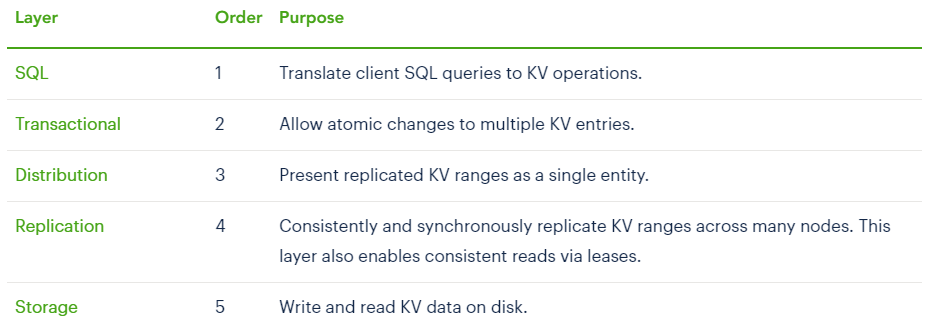
\includegraphics[width=\textwidth]{layers}
    \caption{Table of all layers in CockroachDB\cite{cockroach-architecture-overview}}
    \label{fig:layers}
\end{figure}

\begin{figure}[H]
	\begin{center}
		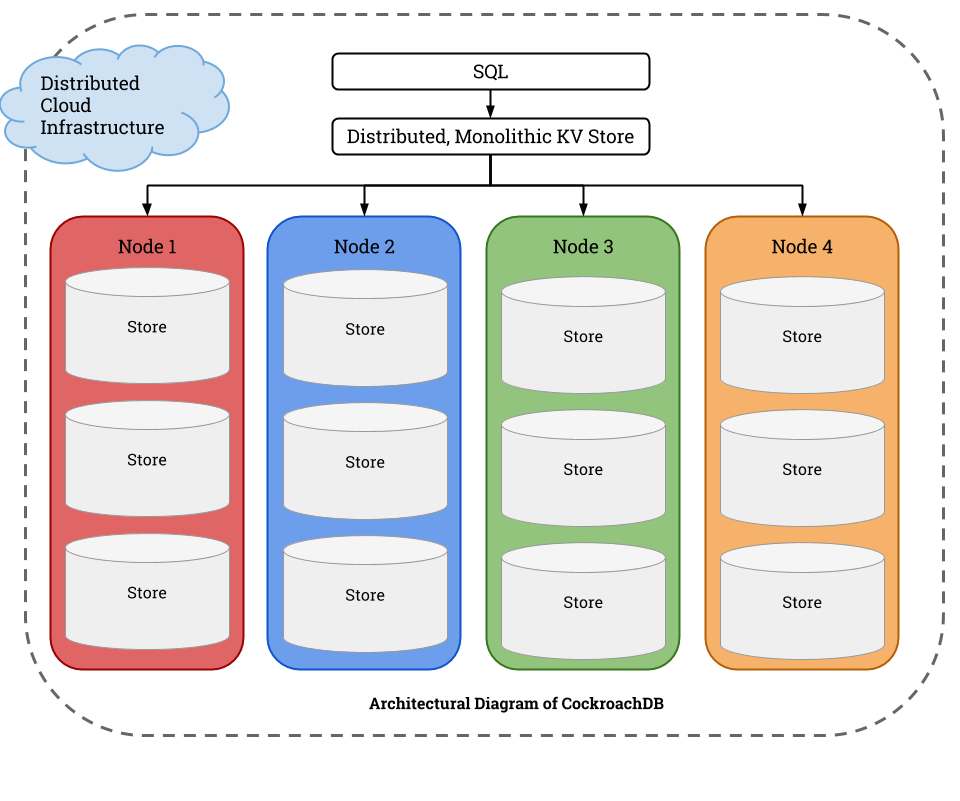
\includegraphics[scale=0.25]{architecture-diagram}
	\end{center}
    \caption{Diagram of CockroachDBs layered architecture\cite{cockroach-newstack}}
    \label{fig:architecture-diagram}
\end{figure}

\paragraph{Nodes}
are a collection of many stores. In reality they can be either physical or virtual machines.

\paragraph{Stores}
are the smallest possible physical unit. It's managed with RocksDB, an open source embedded key-value database.

\subsection{SQL Layer}
\emph{author: Emanuel Kranjec}\bigskip

To support working with relational data CockroachDB provides a SQL layer.\\ \\
With the support of the SQL API developers are able to run familiar SQL queries. When running those statements the cluster gets an request, which initiates to write or read the particular data ultimately as key-value pairs into the storage layer.
Therefore the layer converts beneath the surface these SQL statement into a load of key-value operations, which get processed by the next layer called transaction layer.\\ \\
Developers are even capable of choosing to which node a request should be sent. The receiving node can either process the request or it acts just as so-called gateway node. This is possible because CockroachDB's nodes behave symmetrically. Thus the use of load balancers has ideal prerequisites.

\subsubsection{Relational Structure}
One of the headline features of CockroachDB is the relational structured data storage. The data is organized in rows, columns, tables and even multiple databases. This ensures that relational key features like constraints are supported. Application developers don't need to built data validation into the application logic because the database already guarantees consistent data.

\subsubsection{SQL API}
To keep CockroachDB simple to use it implements a SQL API. The API makes use of a large portion of the ANSI SQL standard, but
as usual in other databases too, some SQL features are differently implemented and not all features are supported. \\
Besides the basic CRUD operations CockroackDB offers constraints like 'primary key', 'foreign key', 'unique', 'not null' and
many more.

\myparagraph{Transaction}
Even transactions are available to keep the database consistent. Until now CockroachDB has tried many approaches to guarantee
ACID transactions. The previous concept was a serializable, lockless and distributed strategy. 
The problem with the lockless design was that it couldn't sufficiently guarantee consistency. Therefore this design was 
discarded. To provide serializable isolation it's now a more locking and lock-like structure. 
More information to this topic is in the transaction layer chapter.

\myparagraph{Joins}
As implementing efficient join algorithms is a big challenge in distributed SQL CockroachDB released since 2016 
constantly new and improved implementations.
CockroachDB currently supports ’merge joins’, ’hash joins’ and ’lookup joins' algorithms in production and additionally
{’lateral joins’} (a type of correlated subquery) since version 20.1 alpha.
The launch of the hash join algorithm in 2017 reduced the asymptotic time complexity from previously O(N*M) to O(N+M).
Later on the merge join algorithm got vectorized because the traditional sort-merge-join \begin{quote} 'fails to take into 
account the overhead of integrating this algorithm into a system. Due to the nature of how data is stored and the interfaces 
used to process the data within the database, there are a few key factors that make this algorithm behave slower in practice 
than in theory. 

In a database, each row of data is encoded in a format that is optimized for a specific purpose, which may 
not necessarily be the same purpose across all cases. To be specific, the current state of the row by row engine stores each 
column of every row in something called a datum. To be able to compare this datum to another datum, there is extra overhead 
in each call to retrieve the value, as first the type of that value has to be determined after which the value has to be 
decoded. Now if this process happens for every single column of every single row, it is clear that isn’t the most efficient 
use of processor time.

Instead, it would make sense if the type check and conversion could happen once per column, since every value in the column 
has the same type. This is called vectorized execution, since the idea is to operate on values a column at a time.'\cite{cockroach-vectorizing-joiner}
\end{quote}
\newpage
\begin{figure}[H]
	\begin{center}
		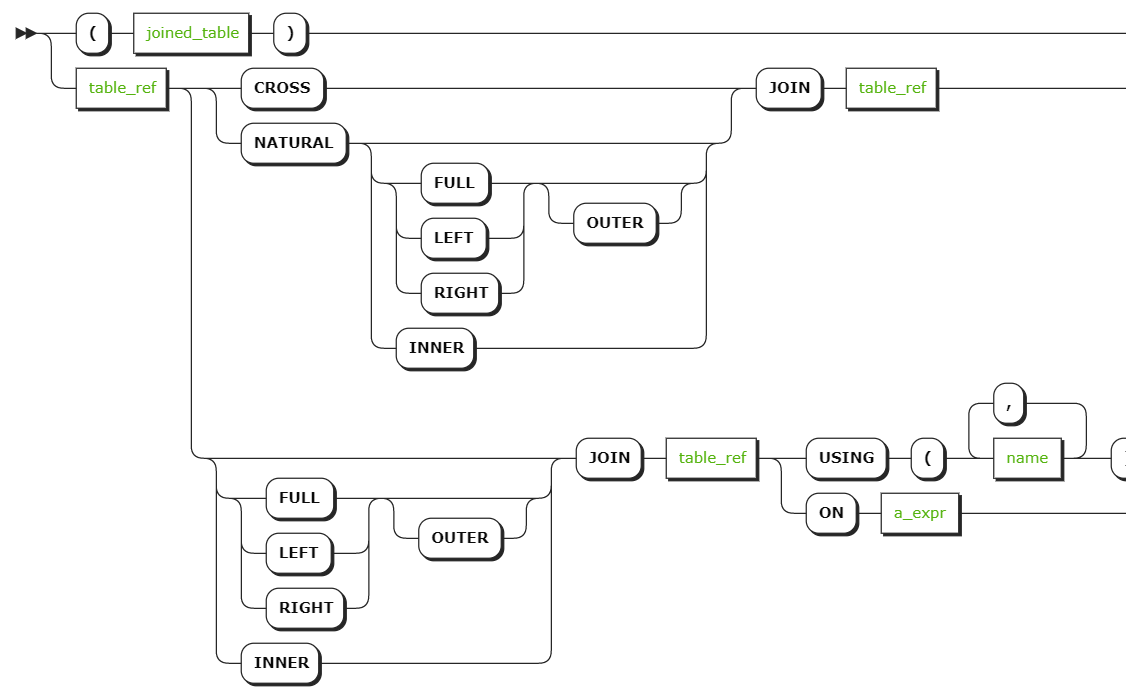
\includegraphics[width=\textwidth]{synopsis-join}
		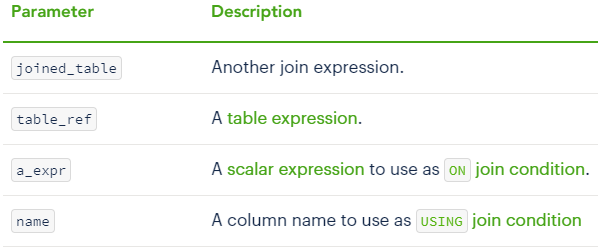
\includegraphics[scale=0.5]{join-parameter}
	\end{center}
    \caption{Synopsis of joins\cite{cockroach-sql-joins}}
    \label{fig:synopsis-join}
\end{figure}



\subparagraph{Inner joins}
\begin{quote}
'Only the rows from the left and right operand that match the condition are returned.'\cite{cockroach-sql-joins}
\end{quote}
\code{
	<table expr> [ INNER ] JOIN <table expr> ON <val expr>\\
	<table expr> [ INNER ] JOIN <table expr> USING(<colname>, <colname>, ...)\\
	<table expr> NATURAL [ INNER ] JOIN <table expr>\\
	<table expr> CROSS JOIN <table expr>
}

\subparagraph{Left outer joins}
\begin{quote}
'For every left row where there is no match on the right, NULL values are returned for the columns on the right.'\cite{cockroach-sql-joins}
\end{quote}
\code{
	<table expr> LEFT [ OUTER ] JOIN <table expr> ON <val expr>\\
	<table expr> LEFT [ OUTER ] JOIN <table expr> USING(<colname>, <colname>, ...)\\
	<table expr> NATURAL LEFT [ OUTER ] JOIN <table expr>
}

\subparagraph{Right outer joins}
\begin{quote}
'For every right row where there is no match on the left, NULL values are returned for the columns on the left.'\cite{cockroach-sql-joins}
\end{quote}
\code{
	<table expr> RIGHT [ OUTER ] JOIN <table expr> ON <val expr>\\
	<table expr> RIGHT [ OUTER ] JOIN <table expr> USING(<colname>, <colname>, ...)\\
	<table expr> NATURAL RIGHT [ OUTER ] JOIN <table expr>
}

\subparagraph{Full outer joins}
\begin{quote}
'For every row on one side of the join where there is no match on the other side, NULL values are returned for the columns on the non-matching side.'\cite{cockroach-sql-joins}
\end{quote}
\code{
	<table expr> FULL [ OUTER ] JOIN <table expr> ON <val expr>\\
	<table expr> FULL [ OUTER ] JOIN <table expr> USING(<colname>, <colname>, ...)\\
	<table expr> NATURAL FULL [ OUTER ] JOIN <table expr>
}\\

The whole table of supported SQL features is \href{https://www.cockroachlabs.com/docs/stable/sql-feature-support.html}{here}\cite{cockroach-sql-feature-support}.

\newpage
\subsection{Transaction Layer}
\emph{author: Emanuel Kranjec}\bigskip

In CockroachDB ACID transactions are fully supported in order to provide consistency. To ensure this every statement in 
CockroachDB is basically a transaction because by default 'autocommit mode' is enabled. Furthermore there is an own protocol
to handle those transactions cross-range and cross-table. 'Parallel commit' is the name of the atomic commit protocol and in
combination with transaction pipelining it reduces significantly the latency of such operations.

\subsubsection{Writing and reading}
To provide consistency in distributed transactions CockroachDB creates write intents and a transaction record.

\paragraph{Write intents} provide the uncommited transaction writes to other tables/ranges like the multi-version concurrency 
control (MVCC) protocol and additionally a pointer to the transaction record. If there is a write intent which handles the
same key there's a transaction conflict. Those write intents can be encountered by future operations while looking for 
MVCC values. The operation knows how to handle the write intent value by checking its transaction record. If there is no 
transaction record it decides based on the timestamp the validity of the write intent.

\paragraph{Transaction record} stores the state of the transaction (PENDING, STAGING, COMMITED, ABORTED) and an array of
writes from this transaction. Thus other transactions can check if this one is already commited and therefore in an
consistent state.

\subsubsection{Parallel commits}
Depending on the state of the transaction record CockroachDB commits or restart the transaction. If the transaction record
says it is in 'STAGING' state the transaction gets checked on whether it is successfully replicated across the cluster. 
If that is true the cleanup phase begins by changing the transaction record state to 'COMMITED', resolving the write intents 
to MVCC values and deleting afterwards these writes.

\subsubsection{Isolation levels}
Even though there are many ANSI transaction levels, CockroachDB decided to only support the 'SERIALIZABLE' level.
This decision is based on a research paper from 2017, named \href{http://www.bailis.org/papers/acidrain-sigmod2017.pdf}
{'ACIDRain: Concurrency-Related Attacks on Database-Backed Web Applications'}\cite{acid-rain-paper} which shows the vulnerability of concurrent 
ACID transactions.\\
Previously the 'SNAPSHOT' level was also supported but the security aspect was valued higher to transaction throughput.

\subsubsection{Transaction conflicts}
CockroachDB handles a transaction conflict by the metrics priority and transaction record.\\\\
When there are for example two write intents which use the same key firstly the priority of there transaction gets compared.
The one with the lower one gets in this case aborted. When the priorities don't differ the transaction which has either no
transaction record or wasn't heartbeated within the transaction liveness threshold gets aborted. If there is still no
decision the write intent which encountered the other one enters the TxnWaitQueue.

\paragraph{Heartbeat} timestamps are there to evaluate if a transaction is abandoned. Active transactions are 
responsible for periodically updating it on its central transaction record. 

\subsubsection{TxnWaitQueue}
As already mentioned in chapter 'Transaction Conflicts' if there is a write/write conflict the last option is to push one
transaction into the TxnWaitQueue. It is a simple map which keeps track of blocking transaction IDs and their blocked 
companions.\\
\graycode{
	txnA -> txn1, txn2
}\\
\graycode{
	txnB -> txn3, txn4, txn5
}
\\The TxnWaitQueue gets manipulated only by the leaseholder which holds the transaction 
records. The queue receives a signal when a transaction got comitted or aborted. Based on this signal it let's particular
transactions execute again.\\
Deadlocks are handled by choosing and aborting a random affected transaction.

\subsubsection{Transaction pipelining}
To reduce latency when making transaction with multiple writes CockroachDB is pipelining those transactions. Pipelining in this
context means all of the affected ranges receive the write intents and write it to the disc in parallel when the transaction got
commited. \\More specifically the gateway node sends the statement to the leaseholders at first and then the leaseholders convert
those statements into write intents. After spreading the write intents within the particular range and receiving confirmations
from all nodes the transaction is considered as commited.\\\\
In the example below the resulting write intents are because of their UUIDs probably in different ranges. This would be an ideal
case because it would be fully parallelized.\\\\
\code{
        BEGIN;\\
        INSERT into kv (key, value) VALUES ('apple', 'red');\\
        INSERT into kv (key, value) VALUES ('banana', 'yellow');\\
        INSERT into kv (key, value) VALUES ('orange', 'orange');\\
        COMMIT;\\
}

\newpage
\subsection{Distribution Layer}
\emph{author: Emanuel Kranjec}\bigskip

To ensure simple and efficient data lookups CockroachDB provides a monolithic sorted map of key-value pairs. Those key-value
pairs include two fundamental elements. One stores the meta range and the other the table data.

\begin{figure}[H]
    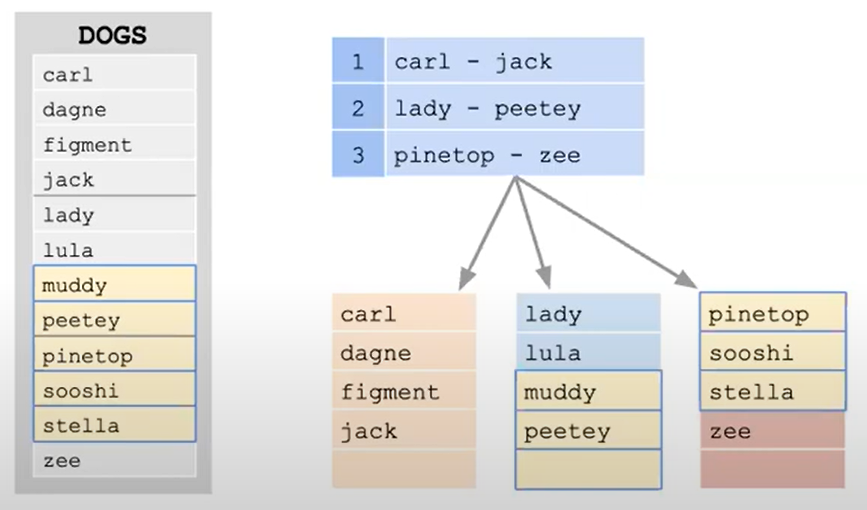
\includegraphics[width=\textwidth]{kv-store}
    \caption{Simplified example of key-values for particular ranges\cite{cockroach-youtube-architecture}}
    \label{fig:kv-store}
\end{figure}

\paragraph{Meta ranges}
describe the location of data including all of its replicas in the cluster.

\paragraph{Table data}
describes the rows of a table included in this particular range.

\newpage
\subsection{Replication Layer}
\emph{author: Felix Tröbinger}\bigskip

CockroachDB consists of a cluster of nodes where each node stores data independently.
CockroachDB stores its data in so called \emph{ranges}. When a range exceeds 64 mebibyte (MiB $ = 1024^2$ bytes) the it is split up into two ranges. Each range is then replicated (the default amount of replication is three) and each one of these replicas is stored on a different node.

\begin{figure}[H]
    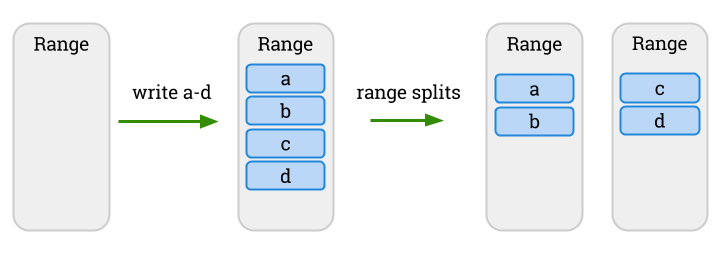
\includegraphics[width=\textwidth]{horizontal-scaling}
    \caption{Range Distribution & Rebalancing in CockroachDB\cite{cockroach-newstack}}
    \label{fig:scaling}
\end{figure}

Figure \ref{fig:scaling} visualizes the range splitting happening in CockroachDB. This happens indefinitely and nodes strive to have a relatively balanced and consistent size.

\medskip
For each range there exists a \emph{leader} who's purpose it is to coordinate read and write access. A leader along with enough followers has to agree before a write action is committed.
Read access don't have to be coordinated with all followers, in this case the leader sends the result to the client without consulting it's followers. This greatly increases performance and speed.
When interacting with CockroachDBs SQL API developers or users can choose to communicate with any given node of the cluster.
If performing a write request on a node that cannot handle the request because it is not the leader, it finds the node who is and is able to fulfill the request.
\cite{cockroach-architecture}

\newpage
\subsection{Storage Layer}
\emph{author: Emanuel Kranjec}\bigskip

Not only the lookup table of the cluster is organized in key-value pairs also the actual data is stored as such. CockroachDB
itself doesn't manage the embedded database storing process.\\
For this purpose they are using the high performance embedded database RocksDB. RocksDB also stores data in the form of 
key-values like CockroachDB does it in the lookup table. Two instaces of RocksDB are on each store. One for holding the write 
intents described in the transaction layer chapter and the other one to store the 
persistent data.\\\\

\begin{figure}[H]
    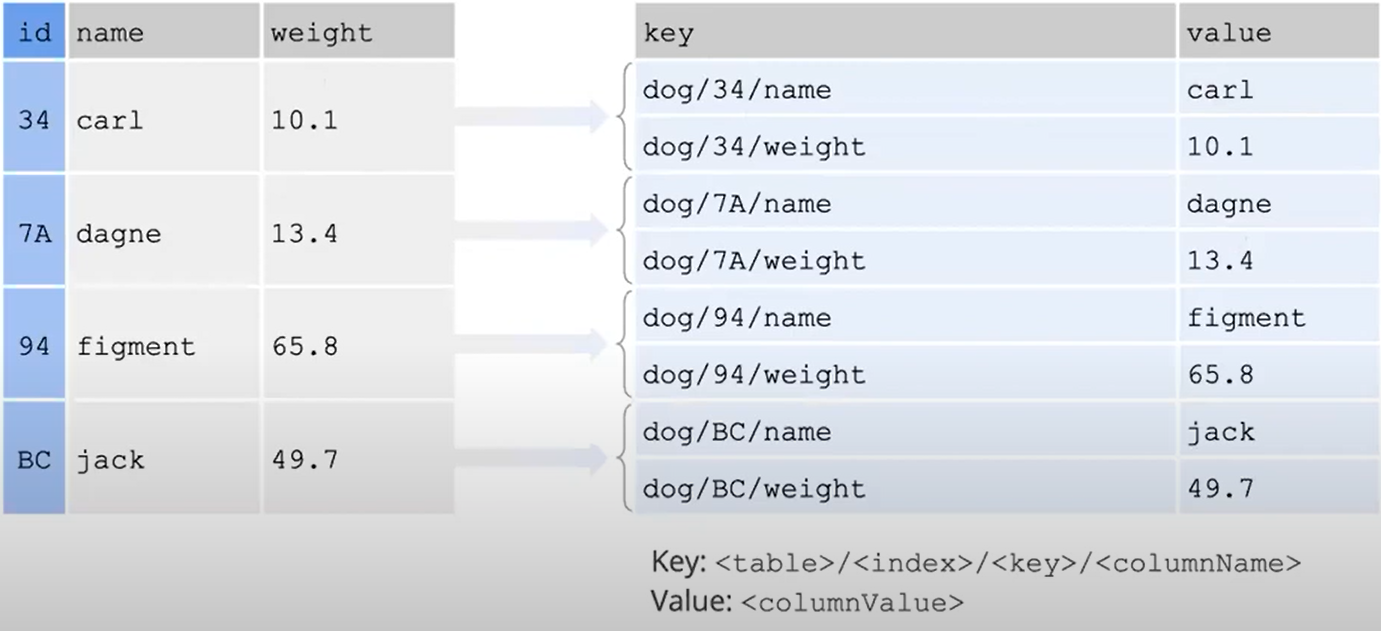
\includegraphics[width=\textwidth]{kv-rocksdb}
    \caption{Conversion of SQL to a key-value store\cite{cockroach-youtube-architecture}}
    \label{fig:kv-rocksdb}
\end{figure}

Furthermore CockroachDB uses MVCC for concurrency purposes. Therefore it is also able to time-travel as described in the SQL:2011 
standard. You can get back as far as the garbage collection got.\\
Garbage collection occurs when a MVCC value exceeds a particular garbage collection period to free memory. The period can be set
from cluster to table level individually.

